\chapter{Introduction}

The term network system passes on, an association of various PCs. For the most part, these systems have two kinds of availability, which are wired and remote. As on account of any innovation, it is development came out as a need. For any country, its most extreme need is to keep up military certainty. The first network system, was the beginning of the era and was essential set up in a military resistance venture called ARPANET, representing the Advanced Research Projects Agency Network. PC arranges throughout the years have developed a wide margin regarding highlights, intricacy, and power. Nowadays, even a layman is familiar to the terms such as switches and routers.

\vspace{5mm}
\section{Traditional Networks}

Even something as new and intense as network systems have demonstrated age. The maturing of innovation is by all accounts a lot snappier than people. Inside two decades, it built up an area of systems known as traditional networks. The spearheading plan of networks is the traditional network. A structure was solid for the time and had no issues for quite a while that was given by Adam Smith of computer networking. Indeed, even now, the traditional network system engineering cannot be blamed as is yet a subject of innovative work. Nevertheless, concerning each innovation that exists, there will be advantages and disadvantages.

\begin{figure}[!hbt]
    \centering
    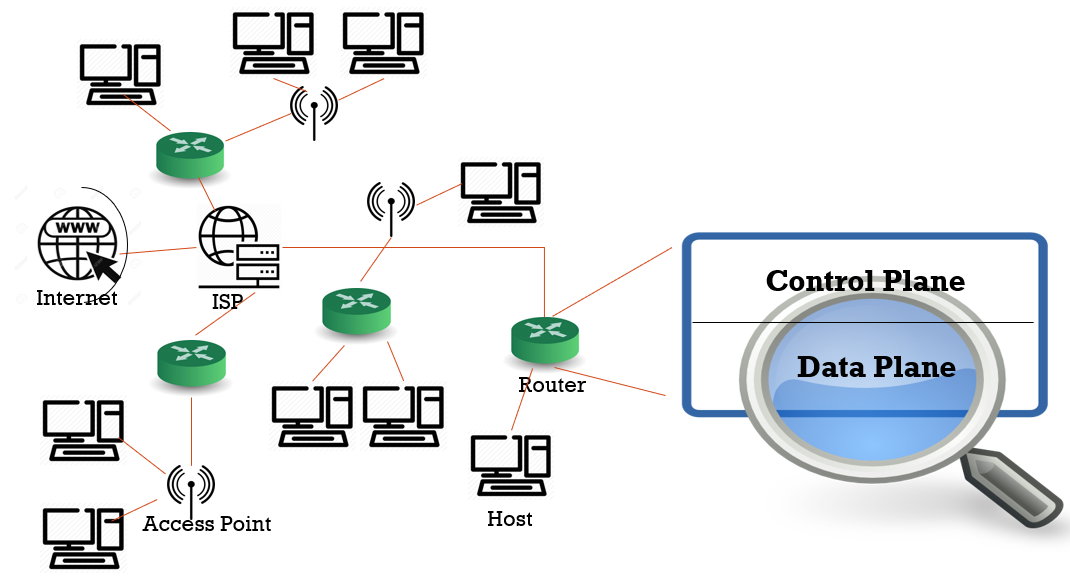
\includegraphics[width=\textwidth,keepaspectratio]{images/TRADITIONAL-NETWORK.png}
    \caption{Traditional Networks \cite{sdnimages}}
    \label{fig:Tradnets}
\end{figure}

   The computer network has been created for the sole purpose of communication. This implies that the advanced data was moved starting with one PC then onto the next remote unit(s), through wire or air. It is proportionate to sending a post starting with one individual then onto the next.
    
    In the case of computer networks, this function of submitting a post is the same and is referred to as routing. No human intervention exists in computer networks; instead, there are independent computers responsible for transmitting this data. Tasks like packet forwarding is assigned to devices that make up a large share in today's global network, called \textit{routers}.
    
    Routers play a vital role in a network, i.e., forwarding packets through specific routes by identifying the current scenario of the neighboring devices and keeping track of the connected devices.  Similar to how someone seems to have a PO box connected to their location, every device in a local area network is listed under a router.  Such routers are dispersed across the network and are necessarily the foundation of the network.  The same explanation is that this method has been tested for years in such a way that it has strong error detection and error correction. Such a network with millions of routing protocol devices ensures redundant information, so there is no single risk. 
    \vspace{2mm}
    
    This routing technique has been used for a long period of time. This will tend to be done for the lifespan of data networks. Across time, routing methods have improved significantly, and numerous techniques and network topologies \cite{topograph1996} have been researched and developed, rendering computer networks even more efficient in modern times. However, simply because something works well does not mean that it can not be improved. Although the debate is not regarding developing routing methods, in particular, it is stressed that the understanding of computer networks is so bland and outdated. The idea of transmitting a data packet with a header added to it to the enormous complexity of the global network appears to bind a message to a carrier pigeon and allow it to ride. Yeah, the pigeon knows how to reach the target by a step-by-step method, but neither the transmitter nor the receiver nor the network administrator knows where the packet is before it enters the informal network where either the recipient or the network administrator is constantly watching and hoping for the packet to arrive.
    
    A simple layout or architecture of the traditional network can be viewed from the Fig. \ref{fig:Tradnets}. There are several small networks connected to a common access point. These access-points are either switches, hubs, bridges or routers. These smaller networks are further connected to a common ISP, which gives these smaller networks access to the Internet.
    
   Packet forwarding is one aspect of the role of the network. Different highlights incorporate observing the system and checking which courses are accessible and which courses are down or under substantial loads with the goal that system traffic can be diverted to another course. Customary systems have some notable answers for such issues; huge numbers of them are ungainly and exploit the assumption that systems administration gadgets are because of quick preparing. They can manage numerous shortcomings simultaneously absent a lot of exertion. Although that might be real, it opens the path to change. Starting at now, there is no single controller to assess the exhibition of the huge system. The switches and routers deal with their immediate neighbours and assume that their neighbours can do likewise. At that point, it was a mind-blowing thought, yet it appears to be excessively simple.
        
    Another model of conventional systems is that every protocol, organize topology or design, expect that the whole network would run a solitary protocol for a lifetime. Then again, as it were, no protocol considered the requirement for versatility or similarity for change contingent upon the situation. A few conventions would adjust to deal with arrange inconsistencies and keep up reliable and unsurprising execution. In any case, the idea of making a network that could change its equipment and programming at some random time was unrealistic.
    
     On account of network issues, there are numerous measures sent to back up and ensure the system can be brought back ready for action. Be that as it may, the acknowledgement of network flaw over the whole network is excessively delayed as far as figuring speeds. In the event that one switch or a server fail someplace in this immense network, the mistake message from its neighbours needs some an ideal opportunity for it to get spread out and diffused to each other gadget in the system. This deferred reaction on account of system deficiencies is something that can be improved.
     
\section{Software Defined Networks}
    
    Traditional networks follow equipment hardware programming engineering. At the end of the day, the systems administration gadgets utilized, for instance, a switch, originated from a particular seller, and the merchant utilizes either their own exclusive programming on it or an outsider programming specially designed for their equipment. Rather, take the instance of a PC. It has equipment produced using a merchant, yet the equipment configuration permits us to introduce any working framework on it and utilize the framework in any methods. Some working frameworks offer more or preferable highlights over some others.
    
     The whole network has an equipment stage which is reasonable for any or different working frameworks one after another. The whole network isn't characterized by the equipment, rather than the working framework that sudden spikes in demand for it and deals with the system.
    
    Such a design as appeared in Fig. \ref{SDNArchitecure} is executed by adopting a concentrated network strategy on decentralized network engineering. The sentence seems like a confusing expression, however, its substance is to broaden the decentralized network engineering by keeping up the data forwarding techniques in its place and on the whole bringing together the system dynamic procedures into a legitimately single element. At the end of the day, the directing usefulness from the switches are evacuated, and they act as switches while making a central element to play out the routing choices and also screen the whole network. This element is named as ''Controller''. This postulation predominantly centres around controllers and the server where it is introduced.
    
    The Fig. \ref{SDNArchitecure} describes the layered architecture of SDN which has basically three distinct abstracted layers namely Application Plane (Application Layer), Control Plane (Control Layer) and Data Plane (Infrastructural Layer). To communicate between these layers, there is use of few APIs like North-Bound API which acts as an interface between Application Plane and Control Plane; South-Bound API acts as an interface between Control Plane and Data Plane. There is use of East-West Bound APIs which acts an interface between its and other Controller's Control Plane.
    
\begin{figure}[!hbt]
    \centering
     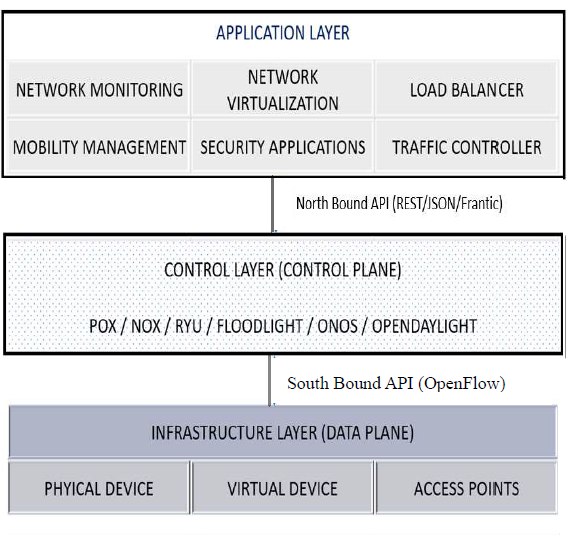
\includegraphics[width=10cm,keepaspectratio]{images/SDN-architecture-example.png}
    \caption{SDN Architecture \cite{sdnimages}}
    \label{SDNArchitecure}
\end{figure}

    Similar to Layer 1 or Physical Layer of OSI Model in Networking, the Infrastructural Layer or Data Plane of SDN Architecture has the main task is to transmit raw bits over a physical data link connected to various network nodes which can be implement either by using a physical or a virtual device. Addition to this, it also has  responsibility of Layer 2 or Data-Link Layer i.e. managing the communications links and handling frame traffic and govern a protocol to access the physical network medium. All these tasks are implemented by use of switches like OpenVSwitch.

    The Control Plane of SDN Architecture can be seen as the Layer 3 or Network Layer of OSI, which is  responsible for packet forwarding including routing through intermediate routers or other nodes. Unlike normal routers, the Control Plane of SDN is implemented at a server rather than on a router. The Control Plane features are established by use of a SDN Controller, an application. Some popular SDN Controllers are Pox, Ryu, Beacon, Nox, Floodlight, ONOS, OpenDayLight, Faucet, RunOS, etc. The Control Plane is also often termed as \textit{Network Operating System}.

    The Application Layer is the top most layer in SDN Architecture where several applications are installed on the server itself and run on top of Controllers via use of various North-Bound APIs build using REST, JSON, or similar languages. Tools like Load Balancers, Network Monitoring, Traffic Controllers, etc are some popular ones in the Application Layer.

    \textit{OpenFlow} is an open and standardized protocol and a flow-based switch specification, which acts as a South-Bound Interface in SDN. It is utilised for collaborating with the sending practices of switches from different merchants. It also control the behavior of switches throughput in a dynamic network and is also programmable. It helps to controller to communicate with switch over a secured channel. It also defines the format of packets.
    
    The corresponding switches are known as OpenFlow Switches. These switches has 3 parts namely an OpenFlow protocol, a flow table, and a secure channel. These switches has the responsibility to forward the flow's packets to given ports or, drop the flow packets or, forward the flow's packets to the controller by encapsulating it.

    As mentioned above, a divide and conquer approach is been followed in the SDN for networking tasks. \cite{taxonomy2014}. In place where every router in the network is performing both the tasks of routing and also of storing these routes to a routing table so to use these routes in future and also to notify the neighboring devices whenever there is a change in network which allows routers to focus on data-forwarding and this also reduces the repetitive calculations of find an optimal route. Whenever there is such new routes, the routers just need to ping the neighbours.
    
    All the functionality like calculation of optimal routes, screening of the topology, or health of the network, are performed by the controllers. This helps to manage the entire network like an interface. This further brings in various benefits to the network like the communication to other middleman devices is no longer needed to know the status of the network. Instead, now there is a central device i.e., Controller(s),  is/are simply dumping all information within itself and thus is making sure whether the network run smoothly or not.

Another preferred position of utilizing a different substance for controlling the system is that it permits the system to be convention autonomous. As it were, the working framework or the software that is running on the controller isn't fixed. The SDN engineering permits to change the working framework at whatever point required. \cite{arpanet2004} In all actuality, it will be a tedious assignment before the system is done and running once more, however it surely is a snappier and less expensive option in contrast to changing the product on all the gadgets in the network.

In any innovation, the prizes will consistently come at either an exchange of or in danger. From moderate yet advantageous transportation of the bike to the marvellous however hazardous aeronautics innovations, improvement consistently includes some significant downfalls. So also, in SDN too, there are a few bills to be paid. 

Right off the bat, the execution of an aggregate substance called the controller is impeding placing all investments tied up on one place. This technique, anyway productive, despite everything, represents a hazard. The general guideline in any administration innovation is to build excess. In the event that, for sizeable SDN, there is a solitary controller, if there should arise an occurrence of any deficiencies running from power blackouts to disastrous events can make the whole system come up short.

    Another drawback of SDN is that the focal controller doesn't really screen the genuine traffic itself rather just the network's well-being and various routes. It doesn't really screen the traffic is on the grounds that controllers are equipped for checking network traffic-utilizing outsider applications. It is truly feasible for the controller to constantly ping a switch so as to get the parcels it handles and read its substance. Be that as it may, it is unbelievably illogical, and along these lines seeking after such an element would yield fewer returns than the exertion put in. So normally, designers don't concentrate on traffic checking as much when contrasted with organizing observing and steering. This fundamentally diminishes the extent of SDN as systems in which traffic can't be observed effectively would represent a hazard as far as genuineness and security. Except if the whole network is trusted by the system manager and the network members, such a technique would appear to be less liked.
    
    To wrap things up, as an expansion to the focuses preceding the past one, since a solitary element controls the whole system's directing and screens the system well-being and topology, this will clearly bring about an extreme overhead on the controller. It was referenced that SDN networks are working framework autonomous, however they are, as it were, reliant on the equipment confinements. For example, processing power, bandwidth , and will keep the network from developing past an outright scale. As the network scales up, so does the complexity in taking care of such a broad network. Routing, topology discovery, etc., becomes awkward except if the controller equipment is updated.\cite{netflow2004}
    
    Additionally, this makes the network versatile, which means it will in general need to come back to its unique measurements, due to overemphasizing on the controller. Except if the controller is changed, which, despite the fact that not so costly or tedious, creates a level of lack of quality in the system, in traditional networks, load adjusting on routes would be performed by neighbouring routers, and the undertaking of network checking was assigned, this implied the network overhead could never go past a cutoff. In the event that all the switches in the network arrived at its cutoff, only including more switches and separating huge networks to littler subnets would be sufficient. Nonetheless, that is unsure on account of programming characterized systems. Circulated controllers take care of this issue to a degree, yet at the same time need more opportunity to form into an increasingly hearty methodology.
    
    \section{Motivation \& Problem Statement}
    
    SDN or Software Defined Networking brings an another point of view to organize networks. The idea of having a concentrated way to deal with decentralized network design brings the benefits of the two models. SDN engineering gives the infrastructural adaptability and vigor of the traditional systems with the additional element of having a central interface to screen and deal with the whole network.
    
    There are many SDN implementations, each with a different controller operating system. However, there comes a question to choose the suitable controller for a network scenario where there are limited resources. Here, controllers are analyzed and tested for system-level performance metrics under a massive network traffic that appears similar to real-world networks. It helps to identify system-level bottlenecks of the controllers and makes it possible to classify controllers based on their system performances. It also generates the idea of whether the provided system is suited to a given controller and vice-versa.